

\begin{frame}{Unsupervised Text Analysis}

  \begin{columns}
    \column{.3\linewidth}
      \gfx{chinese}{.9}
    \column{.3\linewidth}
      \gfx{white_house}{.9}
    \column{.3\linewidth}
       \begin{center}
         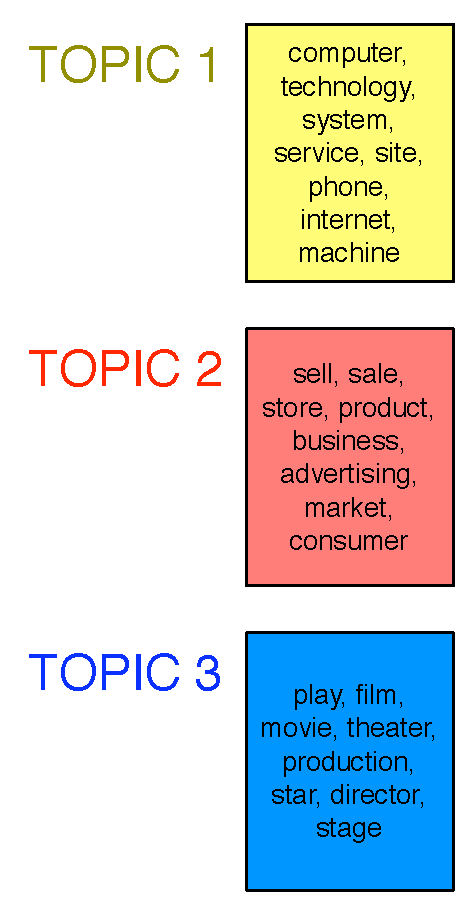
\includegraphics[width=.9\linewidth]{topic_models/nyt_topics}
       \end{center}
  \end{columns}


\end{frame}


% UNSUPERVISED LEARNING: We want to find patterns in text
% - what's a word?
% - What are topics?
% - what are collocations?
% - what's induced grammar
% Common problem: they're hard

\begin{frame}{Problem\onslide<5->{---Scalability Bottleneck}}
  \vspace{-3mm}
  \begin{center}
    \only<1>{
      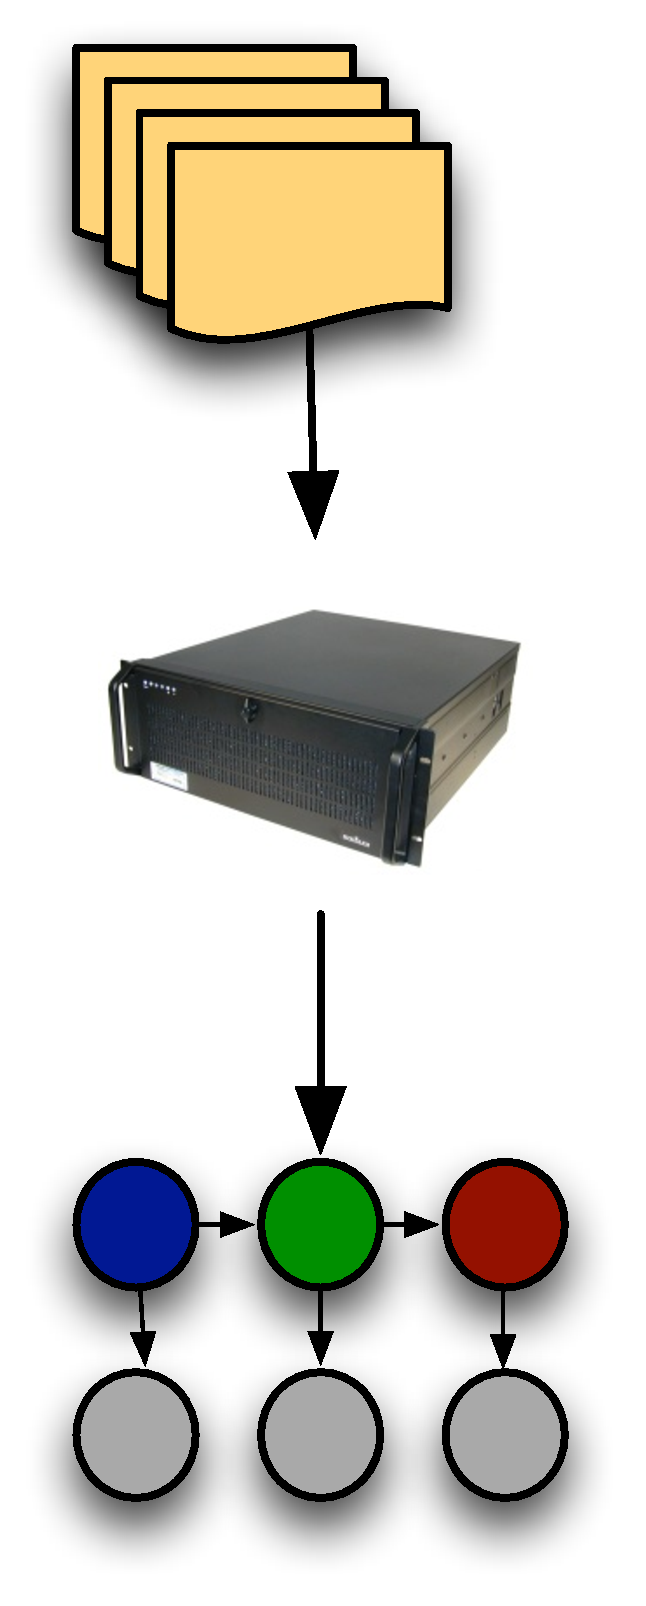
\includegraphics[height=.6\linewidth]{onlineag/batch-1-crop}
    }
    \only<2>{
      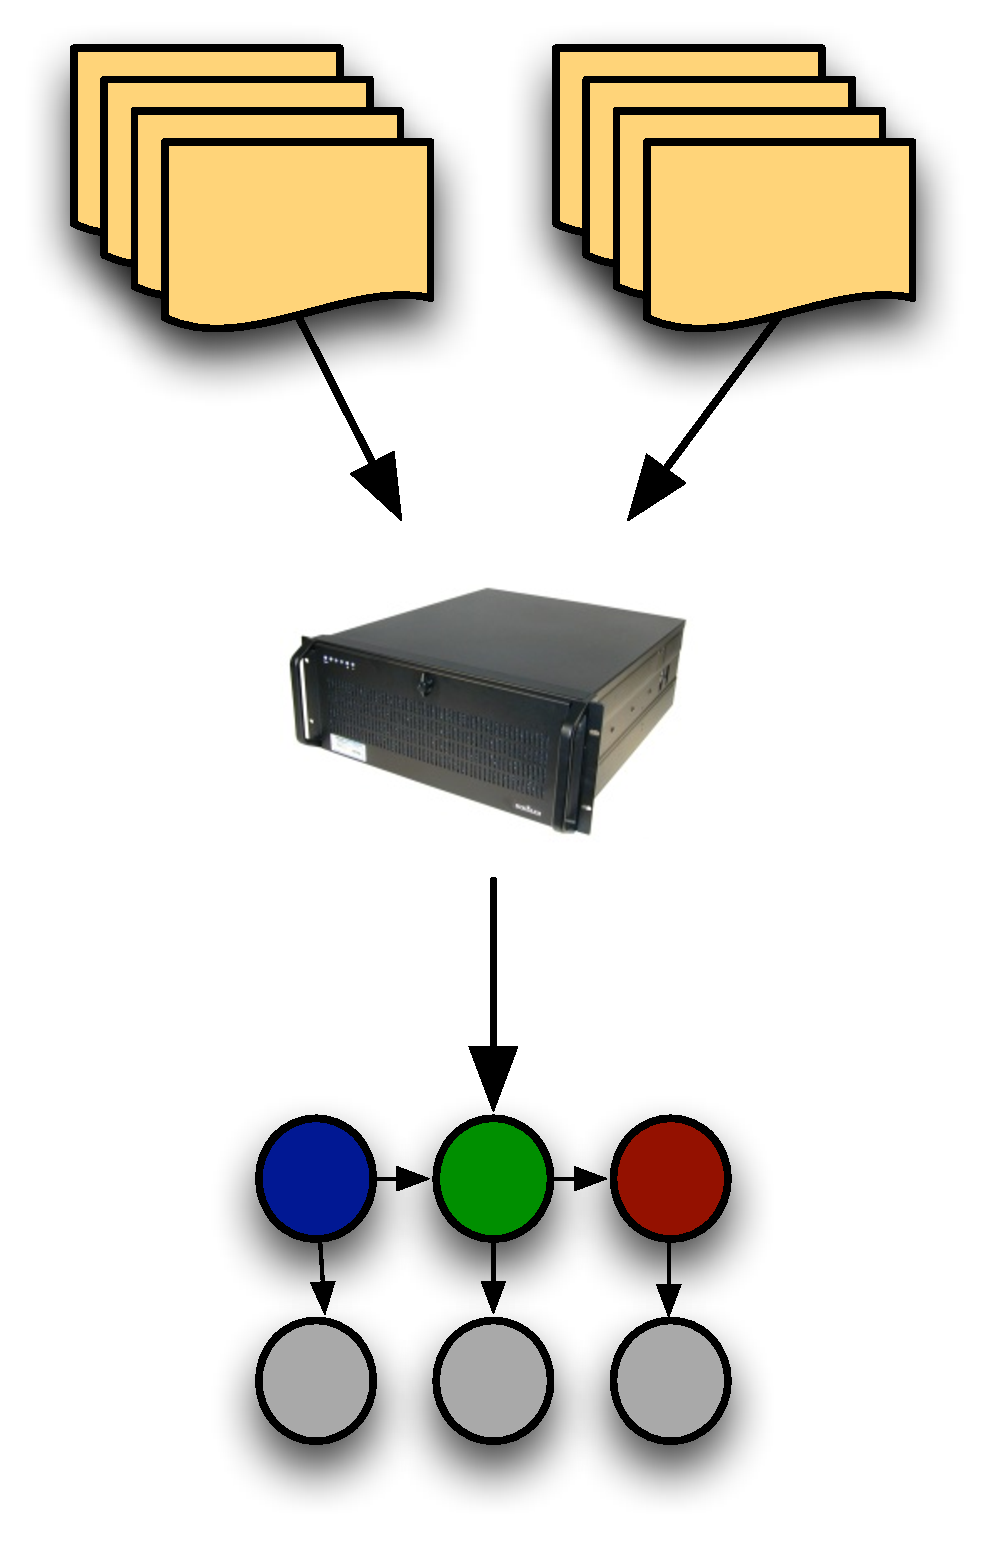
\includegraphics[height=.6\linewidth]{onlineag/batch-2-crop}
    }
    \only<3>{
      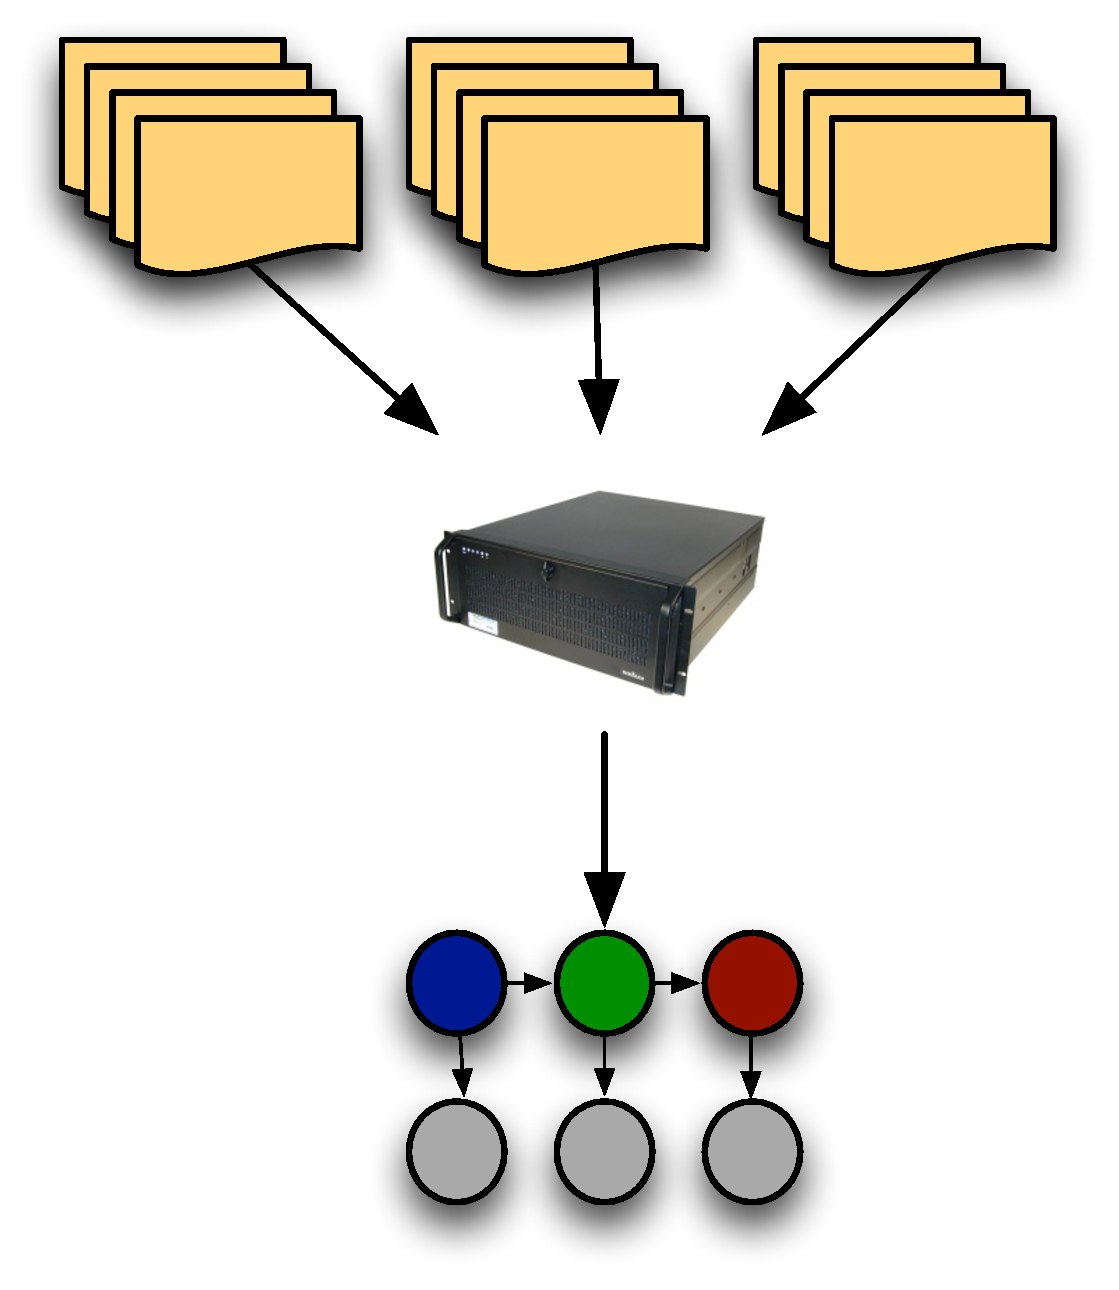
\includegraphics[height=.6\linewidth]{onlineag/batch-3-crop}
    }
    \only<4>{
      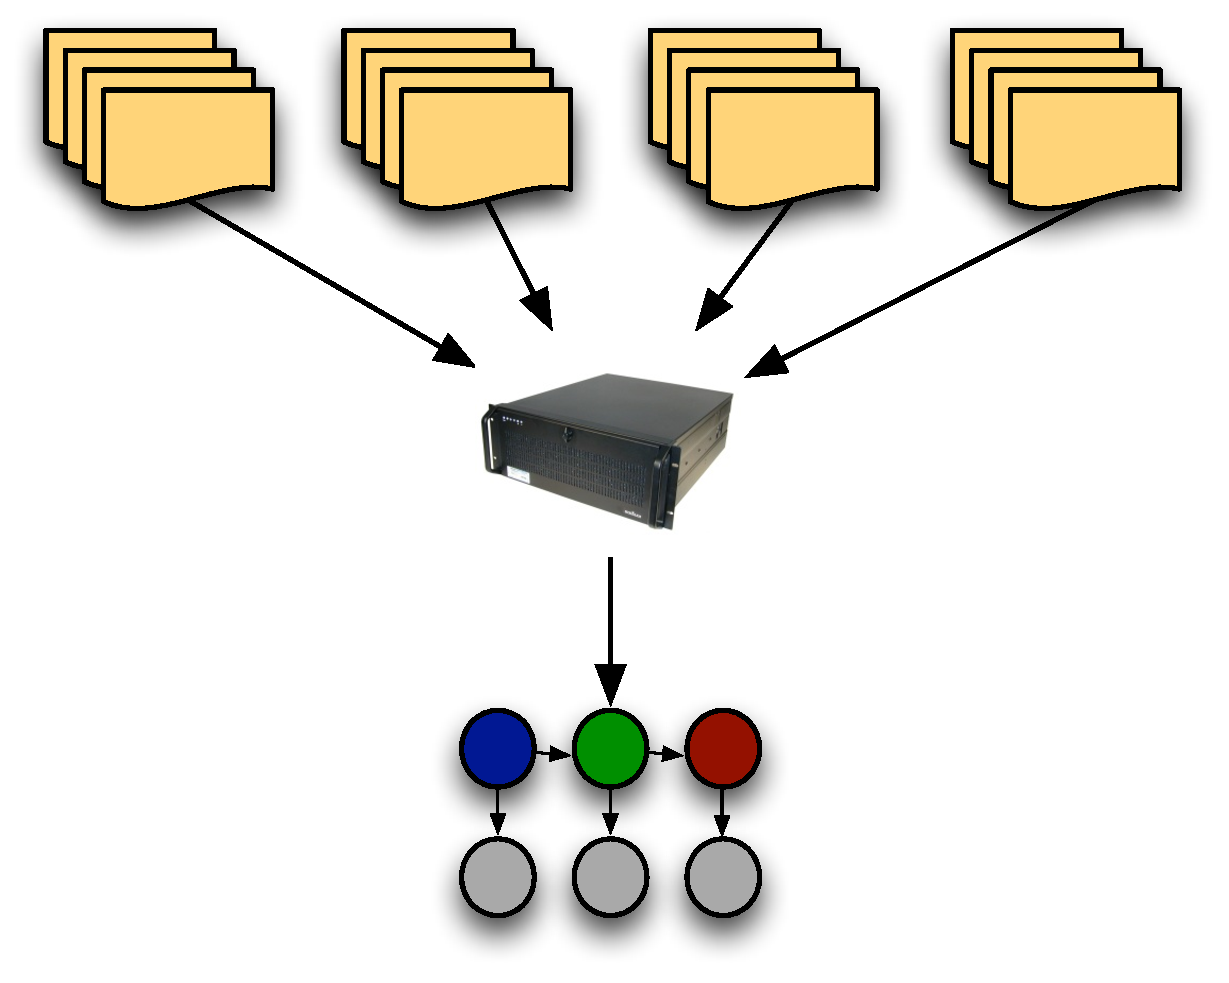
\includegraphics[height=.6\linewidth]{onlineag/batch-4-crop}
    }
    \only<5>{
      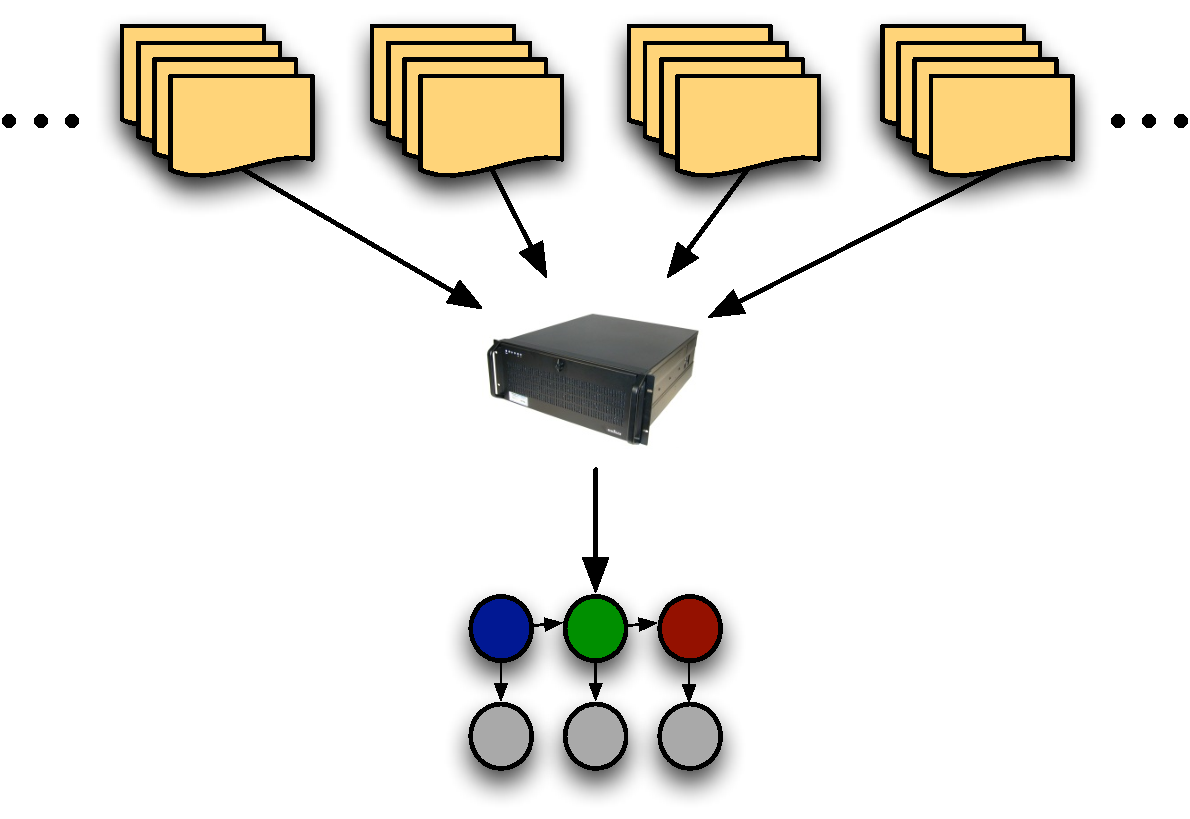
\includegraphics[height=.6\linewidth]{onlineag/batch-5-crop}
    }
    \onslide<5>{
      \\
      Batch algorithms can't scale to large dataset!
    }
  \end{center}
\end{frame}

\begin{frame}{One Solution: Parallelization}
  \begin{center}
    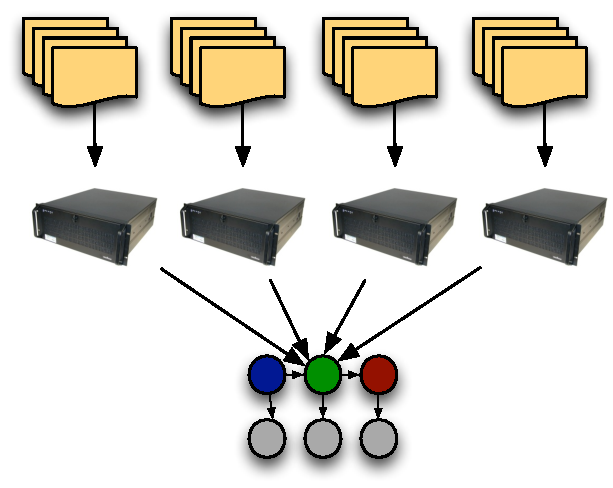
\includegraphics[width=.7\linewidth]{onlineag/parallel} \\
    Throw more computers at the problem%~\citep{smola-10}
  \end{center}
\end{frame}

\begin{frame}{Another Solution: Streaming Algorithms}
  \begin{center}
    \only<1>{ 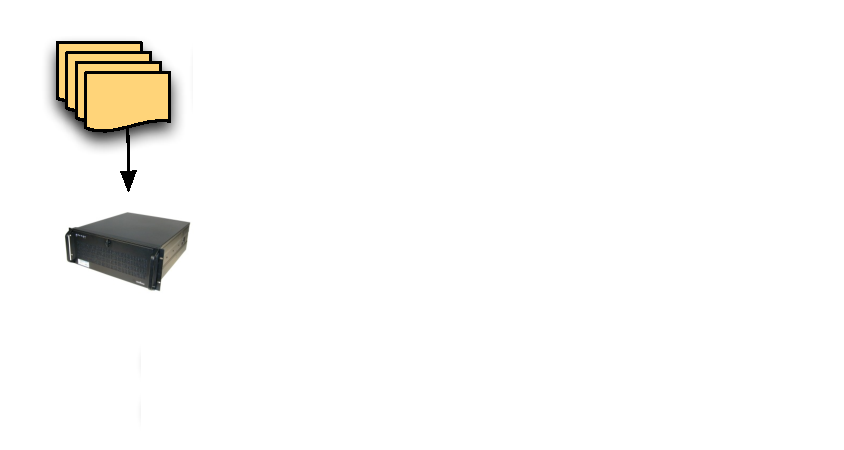
\includegraphics[width=.8\linewidth]{onlineag/streaming-0}}
    \only<2>{ 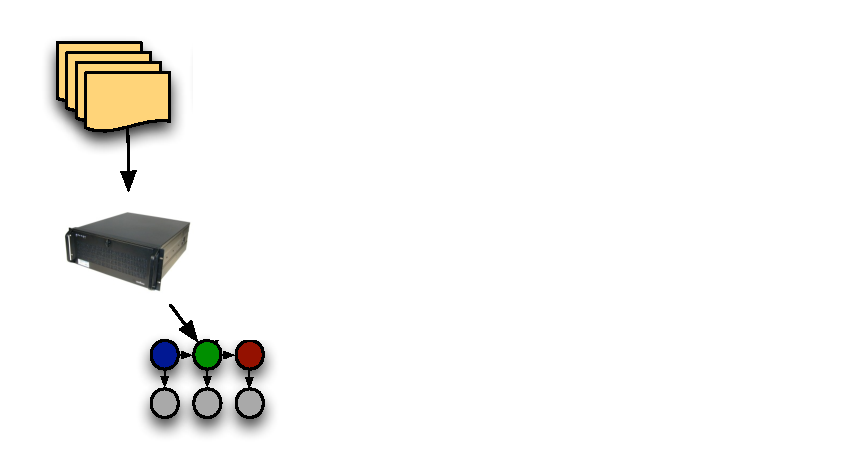
\includegraphics[width=.8\linewidth]{onlineag/streaming-1}}
    \only<3>{ 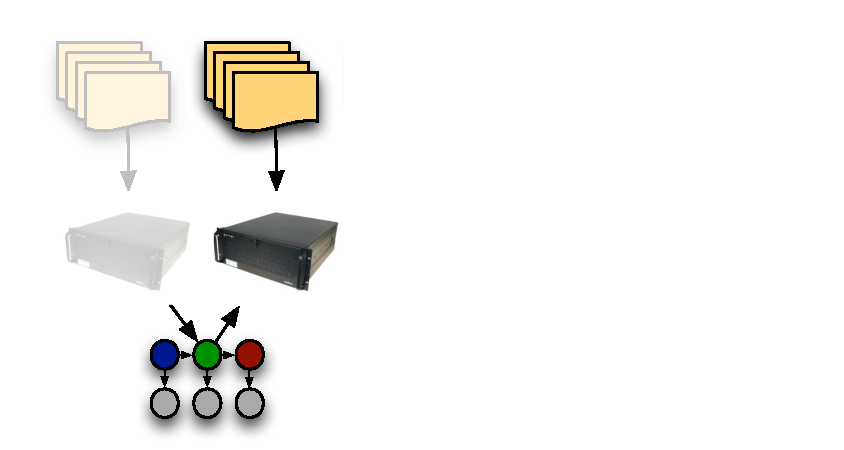
\includegraphics[width=.8\linewidth]{onlineag/streaming-2}}
    \only<4>{ 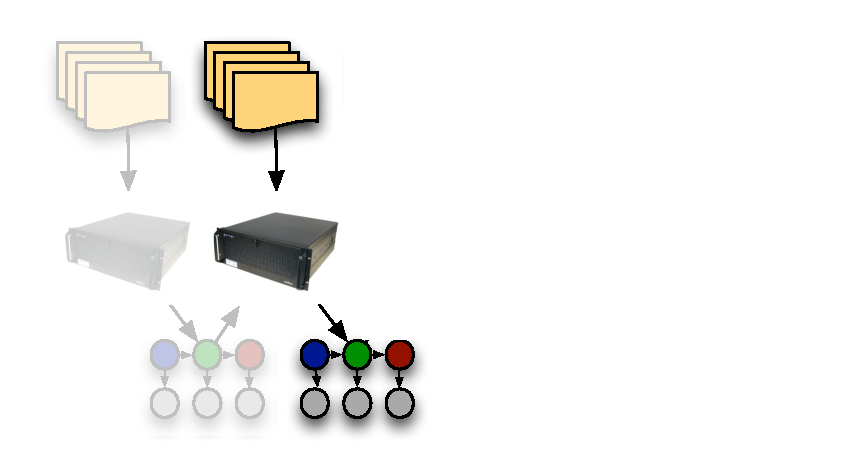
\includegraphics[width=.8\linewidth]{onlineag/streaming-3}}
    \only<5>{ 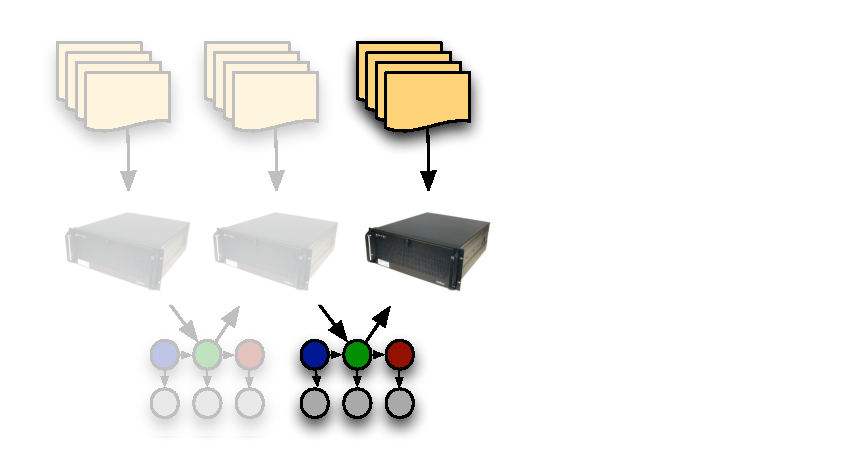
\includegraphics[width=.8\linewidth]{onlineag/streaming-4}}
    \only<6>{ 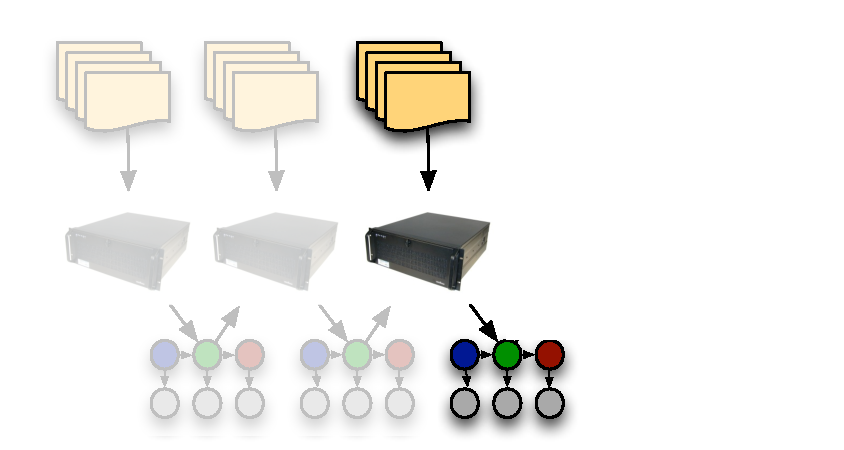
\includegraphics[width=.8\linewidth]{onlineag/streaming-5}}
    \only<7>{ 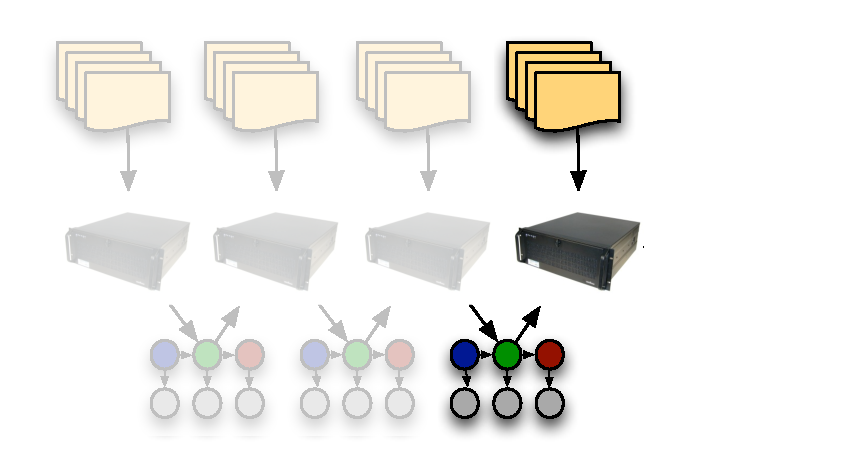
\includegraphics[width=.8\linewidth]{onlineag/streaming-6}}
    \only<8>{ 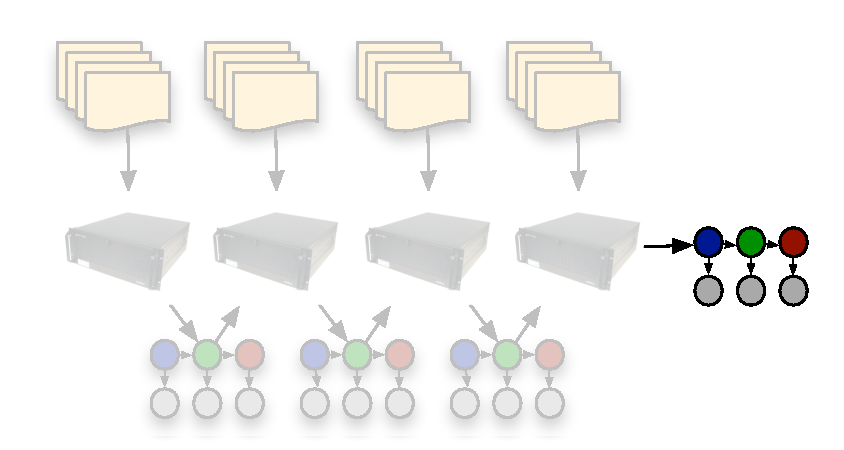
\includegraphics[width=.8\linewidth]{onlineag/streaming-7}}
    \\
    Handle the data as they come.\\
    Process one \alert<1-8>{mini-batch} at one time.
  \end{center}
\end{frame}
